\documentclass[12pt]{article}

\usepackage{sbc-template}
\usepackage{graphicx,url}
\usepackage[utf8]{inputenc}
\usepackage[brazil]{babel}
\usepackage{booktabs}
\usepackage{multirow}

\sloppy

\title{LendingRisk AI: Estimativa do Risco de Perda em Empréstimos\\
  com Aprendizado de Máquina e Explicação por LLM Local}

\author{Hyan da Cunha Ferreira Inácio\inst{1}, Luan Ibanhez de Almeida\inst{1}}

\address{Instituto Federal de Educação, Ciência e Tecnologia de São Paulo (IFSP)\\
  Câmpus Caraguatatuba -- Caraguatatuba -- SP -- Brasil
  \email{\{EMAIL-HYAN, EMAIL-LUAN\}@aluno.ifsp.edu.br}
}

\begin{document}

\maketitle

\begin{abstract}
  This paper presents LendingRisk AI, an academic prototype that estimates the
  probability that a loan ends as a loss (\textit{Charged Off}) using historical
  Lending Club data, and uses a local Large Language Model (LLM) to explain the
  result in Portuguese. We trained Logistic Regression, Random Forest and XGBoost
  on 673,553 matured loans (2007--2015) with a temporal split and ten
  application-time features. A maturity filter was required to avoid selection
  bias in recent cohorts. XGBoost was selected by Average Precision on validation
  and reached, on the held-out test set, AP of 0.243 (random baseline 0.148),
  ROC-AUC of 0.662 and good calibration (ECE of 1.5 percentage points). The LLM
  only verbalizes the classifier output, guarded by an automatic consistency check.
\end{abstract}

\begin{resumo}
  Este artigo apresenta o LendingRisk AI, protótipo acadêmico que estima a
  probabilidade de um empréstimo terminar como perda (\textit{Charged Off}) a
  partir de dados históricos do Lending Club e usa uma LLM local para explicar o
  resultado em português. Regressão Logística, Random Forest e XGBoost foram
  treinados com 673.553 empréstimos encerrados (2007--2015), divisão temporal e
  dez atributos conhecidos no momento do pedido. Um filtro de maturidade foi
  necessário para evitar viés de seleção nas safras recentes. O XGBoost,
  escolhido pela \textit{Average Precision} (AP) na validação, obteve no teste
  reservado AP de 0,243 (contra 0,148 do acaso), ROC-AUC de 0,662 e boa
  calibração (ECE de 1,5 p.p.). A LLM apenas redige o resultado do classificador,
  sob verificação automática de consistência.
\end{resumo}


\section{Introdução}

A concessão de crédito depende de estimar, antes da assinatura do contrato, a
chance de o tomador não honrar a dívida. Modelos estatísticos de \textit{credit
scoring} são usados há décadas para essa tarefa \cite{thomas2017credit}, e
técnicas de Aprendizado de Máquina (AM), como florestas aleatórias e
\textit{gradient boosting}, aparecem com frequência em comparações recentes
\cite{lessmann2015benchmarking}. Em plataformas de empréstimo entre pessoas
(\textit{peer-to-peer}), como o Lending Club, o investidor assume diretamente o
risco, o que torna a estimativa ainda mais relevante \cite{serrano2015determinants}.

Uma probabilidade isolada, porém, é pouco compreensível para quem não é da área.
Os grandes modelos de linguagem (\textit{Large Language Models}, LLMs) podem
transformar a saída numérica em texto acessível, mas também podem inventar
números ou causas \cite{ji2023survey}. Em um contexto de crédito, um texto que
contradiz o modelo é pior do que nenhum texto.

Este trabalho descreve o LendingRisk AI, desenvolvido na disciplina Ciência de
Dados e Sistemas Inteligentes do curso de Tecnologia em Análise e
Desenvolvimento de Sistemas do IFSP Caraguatatuba. O sistema integra
pré-processamento de dados, três classificadores e uma LLM executada localmente.
Os objetivos são: (i) estimar a probabilidade de um empréstimo terminar como
\textit{Charged Off} usando apenas informações disponíveis no momento do pedido;
(ii) avaliar os modelos com um protocolo temporal, sem vazamento de dados; e
(iii) explicar o resultado em português sem que a LLM altere ou invente valores.
Trata-se de um protótipo acadêmico, que não deve ser usado para aprovar ou
recusar crédito real. O código, os relatórios e os registros de execução estão
disponíveis publicamente\footnote{\url{https://github.com/luaniban/lendingrisk-ai}}.

O restante do artigo está organizado assim: a Seção~\ref{sec:referencial}
apresenta os conceitos usados; a Seção~\ref{sec:metodologia} descreve dados e
protocolo; a Seção~\ref{sec:resultados} traz os resultados; a
Seção~\ref{sec:discussao} discute limitações; e a Seção~\ref{sec:conclusao}
conclui.


\section{Referencial Teórico}\label{sec:referencial}

\subsection{Classificação binária e desbalanceamento}

O problema é tratado como classificação binária supervisionada: dado um vetor de
atributos de um empréstimo, o modelo estima $P(y=1\mid x)$, em que $y=1$
indica \textit{Charged Off}. Como a classe positiva é minoritária (cerca de 15\%
dos casos), a acurácia é enganosa: prever sempre a classe majoritária já acerta
85\% \cite{he2009learning}. Nesses casos, a curva Precisão$\times$Revocação
(\textit{precision-recall}) é mais informativa que a curva ROC
\cite{davis2006relationship,saito2015precision}. A \textit{Average Precision}
(AP) resume a curva precisão$\times$revocação, e seu valor para um classificador
aleatório é igual à proporção de positivos. A medida $F_\beta$
\cite{vanrijsbergen1979information} combina precisão e revocação; com $\beta=2$,
a revocação recebe peso maior, o que é adequado quando deixar de sinalizar um
mau pagador custa mais que um falso alarme.

\subsection{Calibração}

Além de ordenar bem os casos, um modelo de risco deve produzir probabilidades
coerentes com as frequências observadas. O \textit{Brier score}
\cite{brier1950verification}, erro quadrático médio da probabilidade, e o
\textit{Expected Calibration Error} (ECE) \cite{naeini2015obtaining,guo2017calibration},
diferença média ponderada entre probabilidade prevista e taxa observada por
faixas, medem essa propriedade.

\subsection{Modelos}

A Regressão Logística \cite{hosmer2013applied} é o modelo de referência em
\textit{credit scoring} por sua simplicidade e interpretabilidade. A Random
Forest \cite{breiman2001random} combina árvores de decisão treinadas em amostras
\textit{bootstrap} com subconjuntos aleatórios de atributos. O XGBoost
\cite{chen2016xgboost} é uma implementação eficiente de \textit{gradient
boosting} de árvores, com regularização. Para estimar a importância global dos
atributos, usa-se a importância por permutação \cite{breiman2001random}: mede-se
quanto a métrica piora quando um atributo é embaralhado.

\subsection{Vazamento de dados}

Vazamento (\textit{leakage}) ocorre quando o modelo usa, no treino, informação
que não estaria disponível no momento da previsão \cite{kaufman2012leakage}. Em
crédito, colunas como total pago ou valores recuperados só existem depois da
concessão e tornariam o modelo artificialmente bom. O ajuste do
pré-processamento (imputação, padronização) com dados de validação ou teste é
outra forma de vazamento.

\subsection{LLMs como camada de explicação}

LLMs geram texto fluente, mas podem produzir conteúdo não sustentado pela
entrada, fenômeno conhecido como alucinação \cite{ji2023survey}. Modelos
compactos, como o Llama 3.2 de 3 bilhões de parâmetros
\cite{grattafiori2024llama}, podem ser executados localmente na CPU por meio do
Ollama \cite{ollama}, o que evita enviar dados a serviços externos.
Neste trabalho a LLM é restrita a redigir a saída do classificador, sem acesso ao
modelo e sem papel na decisão.


\section{Metodologia}\label{sec:metodologia}

\subsection{Dados}

Foi usado o arquivo \texttt{accepted\_2007\_to\_2018Q4.csv} do conjunto público
Lending Club \cite{lendingclubkaggle}, com 2.260.701 linhas e 151 colunas de
empréstimos emitidos entre 2007-06 e 2018-12. A integridade do arquivo foi
conferida por SHA-256, registrado junto aos resultados.

O alvo foi derivado de \texttt{loan\_status}: $0=$ \textit{Fully Paid}
(quitado) e $1=$ \textit{Charged Off} (baixado como perda). Os demais estados
(\textit{Current}, \textit{Late}, \textit{In Grace Period}, \textit{Default})
não têm desfecho final e foram excluídos, assim como 2.749 registros marcados
como \textit{Does not meet the credit policy}, que seguiram outra política de
crédito. Restaram 1.345.310 empréstimos com desfecho final, dos quais 19,96\%
são \textit{Charged Off}.

Foram usados dez atributos conhecidos no momento do pedido: seis numéricos
(valor solicitado, renda anual, relação dívida/renda --- DTI, limite inferior
da faixa FICO, consultas de crédito nos últimos seis meses e utilização do
crédito rotativo) e quatro categóricos (prazo, finalidade, situação de moradia e
tempo de emprego). As 20 colunas posteriores à concessão presentes no arquivo,
como \texttt{total\_pymnt}, \texttt{recoveries} e
\texttt{last\_fico\_range\_high}, não são lidas, e um teste automatizado garante
isso. A nota (\texttt{grade}) e a taxa de juros (\texttt{int\_rate}) atribuídas
pelo próprio Lending Club também ficaram de fora por decisão de escopo: elas já
resumem o modelo de risco interno da plataforma, e o objetivo é estimar o risco
a partir dos dados do solicitante.

\subsection{Viés de maturidade}\label{sec:maturidade}

Uma auditoria feita antes de qualquer treino mostrou que as safras recentes
estavam, em sua maioria, em andamento. Entre esses empréstimos, os que já tinham
desfecho eram justamente os que terminaram cedo, com maior proporção de baixas
precoces. A Figura~\ref{fig:coortes} mostra o efeito: nas coortes cujo prazo já
havia terminado, 14,82\% dos finalizados são \textit{Charged Off}; nas coortes
não maturadas, 25,12\%. Uma divisão temporal sem tratamento colocaria essa
população atípica na validação e no teste: sem filtro, a taxa de
\textit{Charged Off} passaria de 18,7\% no treino para 24,9\% na validação, por
efeito de seleção e não de mudança real do risco.

\begin{figure}[ht]
\centering
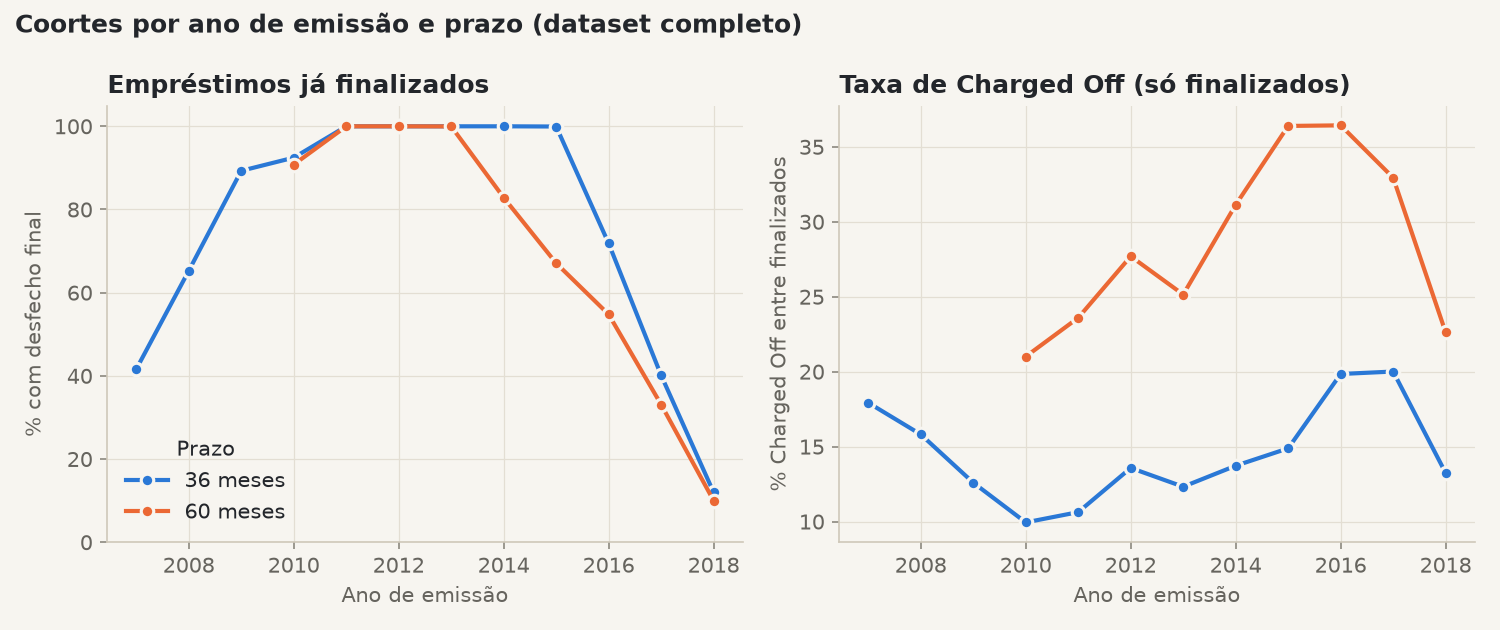
\includegraphics[width=\textwidth]{figuras/auditoria_coortes.png}
\caption{Proporção de empréstimos finalizados (esquerda) e taxa de
  \textit{Charged Off} entre os finalizados (direita), por ano de emissão e prazo.}
\label{fig:coortes}
\end{figure}

Por isso, foram mantidos apenas os empréstimos cujo prazo contratual terminou
até a data de referência do arquivo (\texttt{issue\_d + term} $\leq$ 2018-12).
O filtro removeu 671.757 linhas, e o experimento usou 673.553 empréstimos
(14,82\% de \textit{Charged Off}), toda a população elegível, sem amostragem.

\subsection{Divisão temporal e pré-processamento}

Os dados foram divididos por data de emissão (\texttt{issue\_d}), em cerca de
70\% para treino, 15\% para validação e 15\% para teste, sem que um mesmo mês
aparecesse em duas partições (Tabela~\ref{tab:particoes}). A data de emissão
serve apenas para a divisão e não é atributo do modelo.

\begin{table}[ht]
\centering
\caption{Partições temporais após o filtro de maturidade.}
\label{tab:particoes}
\begin{tabular}{lcrrr}
\toprule
Partição & Período & Linhas & \textit{Charged Off} & Prazo 60 meses \\
\midrule
Treino    & 2007-06 a 2015-04 & 470.714 & 14,81\% & 11,68\% \\
Validação & 2015-05 a 2015-08 &  95.405 & 14,81\% & 0\% \\
Teste     & 2015-09 a 2015-12 & 107.434 & 14,84\% & 0\% \\
\bottomrule
\end{tabular}
\end{table}

O pré-processamento foi encapsulado em um \textit{Pipeline} do scikit-learn
\cite{pedregosa2011scikit}, ajustado somente no treino: imputação pela mediana e
padronização para os atributos numéricos; imputação pela moda e codificação
\textit{one-hot} para os categóricos, ignorando categorias desconhecidas.
Valores extremos foram mantidos.

\subsection{Modelos, seleção e limiar}

Foram treinados três modelos com hiperparâmetros fixos, sem busca:
Regressão Logística (até 1.000 iterações); Random Forest (120 árvores,
profundidade máxima 14, mínimo de 3 amostras por folha); e XGBoost (160
árvores, profundidade 4, taxa de aprendizado 0,08, \textit{subsample} 0,85 e
\textit{colsample\_bytree} 0,9). A semente aleatória foi fixada em 42.

O protocolo foi registrado no repositório antes do treino com os dados reais. O
modelo final é o de maior AP na validação. O limiar de decisão é o que maximiza
$F_2$ na validação, em uma grade de 0,01 a 0,99. O conjunto de teste foi
avaliado uma única vez, com modelo e limiar já escolhidos. Foram calculados AP,
ROC-AUC, Brier, \textit{log loss}, ECE (10 faixas), revocação, precisão, $F_1$,
$F_2$, acurácia e matriz de confusão, além de análises descritivas de
calibração, estabilidade mensal e subgrupos.

\subsection{Interface e LLM}

A interface, feita em Streamlit, recebe os dez atributos e mostra a
probabilidade estimada, o limiar, a classe resultante, as métricas e as
limitações do modelo. A explicação textual usa o modelo \texttt{llama3.2:3b} no
Ollama, executado localmente na CPU, com temperatura 0,1. A LLM recebe a
probabilidade, o limiar, a comparação já calculada (acima ou abaixo) e os
atributos de maior importância global, e devolve um JSON com três frases:
probabilidade, comparação com o limiar e atributos mais usados pelo modelo em
geral. O código monta o parágrafo final.

Uma verificação automática, heurística, confere se a probabilidade e o limiar
foram citados corretamente, se a classe não foi trocada, se o texto foi cortado e
se há atribuição causal (``aumentou o risco'', ``devido a'') ou termos absolutos.
Em caso de erro factual, uma segunda resposta é gerada e mantém-se a com menos
avisos. Se o Ollama não estiver disponível, a interface continua exibindo a
previsão.


\section{Resultados}\label{sec:resultados}

Os experimentos foram executados em um notebook com processador Intel de 8
\textit{threads}, 15~GiB de RAM e sem GPU, com Python 3.12, scikit-learn 1.9.1 e
XGBoost 3.4.1. O treino completo dos três modelos levou cerca de 2,5 minutos e
usou no máximo 1,2~GB de RAM. Três execuções com o mesmo comando produziram
métricas idênticas.

\subsection{Comparação na validação}

A Tabela~\ref{tab:validacao} e a Figura~\ref{fig:pr} comparam os modelos. O
XGBoost teve a maior AP e foi selecionado, com limiar de 0,09. A vantagem é
pequena: +0,004 de AP sobre a Regressão Logística. Com apenas dez atributos, os
três modelos capturam praticamente o mesmo sinal, e a Regressão Logística seria
uma alternativa quase equivalente, mais rápida e mais interpretável.

\begin{table}[ht]
\centering
\caption{Métricas na validação. AP de um classificador aleatório: 0,148.}
\label{tab:validacao}
\begin{tabular}{lrrrrr}
\toprule
Modelo & AP & ROC-AUC & Brier & ECE & Treino (s) \\
\midrule
Regressão Logística & 0,2331 & 0,6529 & 0,1218 & 0,0129 & 3,6 \\
Random Forest       & 0,2323 & 0,6545 & 0,1219 & 0,0158 & 105,5 \\
\textbf{XGBoost}    & \textbf{0,2368} & \textbf{0,6583} & \textbf{0,1214} & \textbf{0,0125} & 6,0 \\
\bottomrule
\end{tabular}
\end{table}

\begin{figure}[ht]
\centering
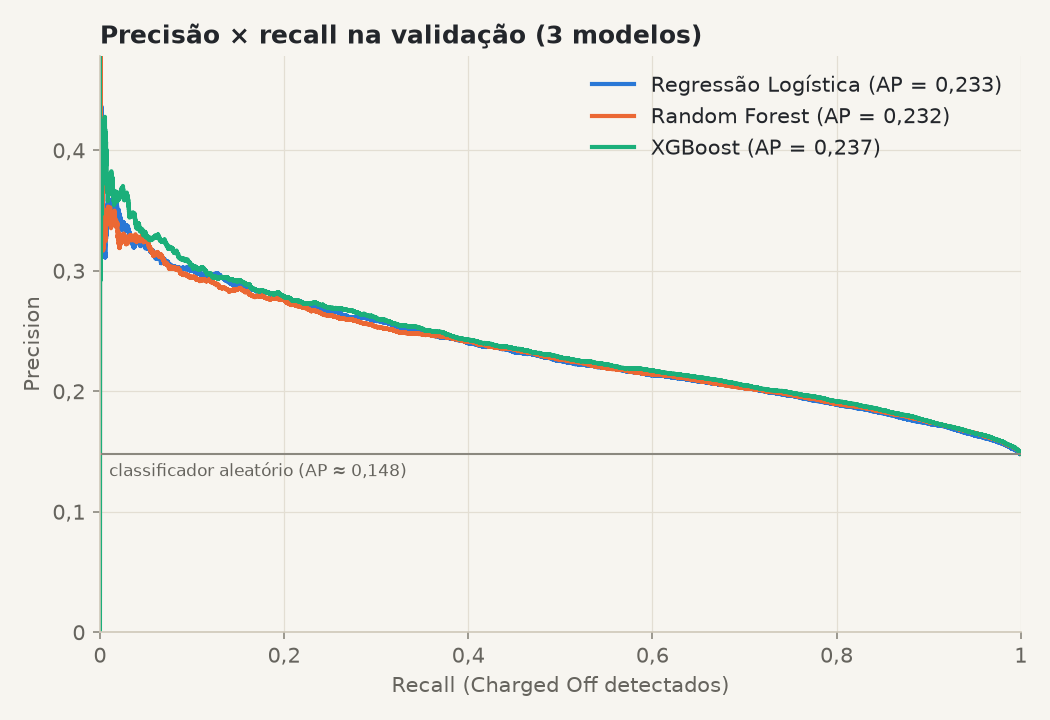
\includegraphics[width=.75\textwidth]{figuras/curvas_pr_validacao.png}
\caption{Curvas precisão$\times$revocação dos três modelos na validação.}
\label{fig:pr}
\end{figure}

\subsection{Avaliação final no teste}

A Tabela~\ref{tab:teste} apresenta o resultado do XGBoost no teste reservado.
A AP (0,2425) supera em 64\% a de um classificador aleatório (0,1484), e o
Brier (0,1214) é menor que o de uma previsão constante igual à taxa observada
(0,1264). Os valores de validação e teste são próximos (AP de 0,237 e 0,243), e
a AP mensal variou entre 0,234 e 0,244 na validação, o que indica estabilidade
no período avaliado.

\begin{table}[ht]
\centering
\caption{XGBoost no teste reservado (107.434 empréstimos, limiar 0,09).}
\label{tab:teste}
\begin{tabular}{lrr}
\toprule
Métrica & XGBoost & Referência trivial \\
\midrule
\textit{Average Precision} & 0,2425 & 0,1484 (aleatório) \\
ROC-AUC                    & 0,6623 & 0,5 \\
Brier                      & 0,1214 & 0,1264 (constante) \\
ECE (10 faixas)            & 0,0155 & --- \\
Revocação                  & 0,8805 & --- \\
Precisão                   & 0,1798 & 0,1484 \\
$F_1$ / $F_2$              & 0,2986 / 0,4948 & --- \\
Acurácia                   & 0,3862 & 0,8516 (sempre \textit{Fully Paid}) \\
Sinalizados como \textit{Charged Off} & 72,68\% & --- \\
\bottomrule
\end{tabular}
\end{table}

A matriz de confusão do teste mostra 14.036 verdadeiros positivos, 1.905 falsos
negativos, 64.043 falsos positivos e 27.450 verdadeiros negativos. O limiar
escolhido por $F_2$ (Figura~\ref{fig:limiar}) é agressivo: sinaliza 73\% dos
empréstimos para capturar 88\% dos \textit{Charged Off}, com cerca de 4,6
falsos alarmes para cada caso detectado. Por isso a acurácia (38,6\%) fica abaixo
da de um classificador que sempre prevê \textit{Fully Paid} (85,2\%), que não
detecta nenhum caso.

\begin{figure}[ht]
\centering
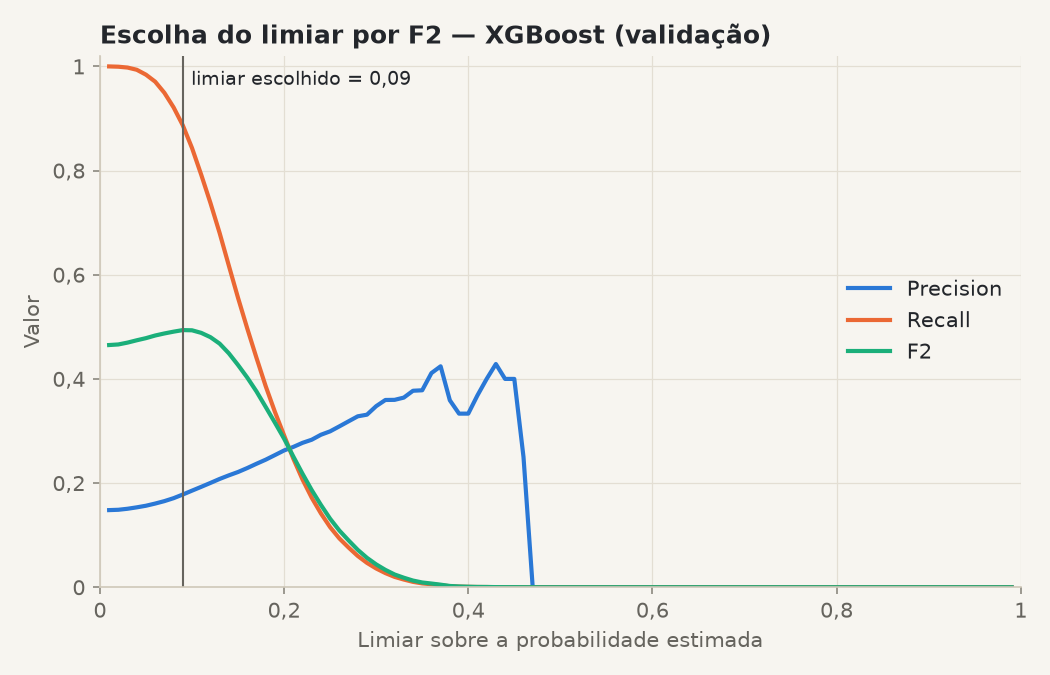
\includegraphics[width=.75\textwidth]{figuras/limiar_validacao.png}
\caption{Precisão, revocação e $F_2$ em função do limiar (XGBoost, validação).}
\label{fig:limiar}
\end{figure}

\subsection{Calibração e importância dos atributos}

A probabilidade estimada é bem calibrada, com ECE de 1,5 pontos percentuais
(Figura~\ref{fig:calibracao}). Há leve subestimação: a probabilidade média
prevista no teste foi 13,3\%, contra 14,8\% observados, e os decis de maior
risco ficam cerca de 2 p.p. abaixo da diagonal. As probabilidades não foram
recalibradas.

\begin{figure}[ht]
\centering
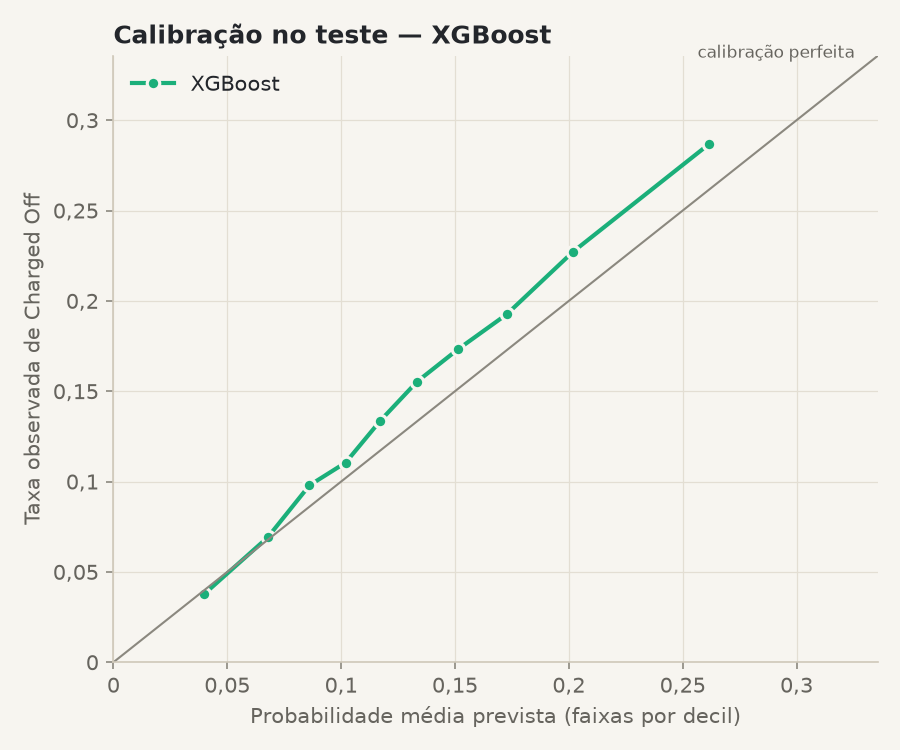
\includegraphics[width=.6\textwidth]{figuras/calibracao_teste.png}
\caption{Curva de calibração do XGBoost no teste, por decis de probabilidade.}
\label{fig:calibracao}
\end{figure}

Pela importância por permutação na validação (queda média de AP), a ordem foi:
faixa FICO (0,027), renda anual (0,017), consultas em seis meses (0,012), valor
solicitado (0,011), finalidade (0,008), DTI e moradia (0,006). O prazo aparece
com importância zero porque a validação só tem empréstimos de 36 meses, o que
não prova irrelevância. Tempo de emprego e uso do rotativo ficaram próximos de
zero, dentro do ruído.

\subsection{Sensibilidade do limiar}

Como análise posterior ao teste, puramente descritiva, foram comparados dois
critérios alternativos de limiar, ambos definidos apenas na validação
(Tabela~\ref{tab:limiares}). Não existe limiar ``correto'': cada escolha troca
\textit{Charged Off} perdidos por falsos alarmes, e a precisão não passa de 26\%
em nenhum deles. O limiar oficial foi mantido, pois havia sido fixado no
protocolo.

\begin{table}[ht]
\centering
\caption{Efeito de critérios de limiar no teste (definidos na validação).}
\label{tab:limiares}
\begin{tabular}{lrrrrrr}
\toprule
Critério & Limiar & Sinaliza & Revoc. & Precisão & Falsos alarmes & CO perdidos \\
\midrule
Máximo $F_2$ (oficial) & 0,090 & 72,7\% & 88,0\% & 18,0\% & 64.043 & 1.905 \\
Máximo $F_1$           & 0,140 & 41,1\% & 60,5\% & 21,9\% & 34.491 & 6.294 \\
20\% de maior risco    & 0,189 & 18,7\% & 32,8\% & 26,0\% & 14.833 & 10.718 \\
\bottomrule
\end{tabular}
\end{table}

\subsection{Análise de erros por subgrupo}

A análise por subgrupos no teste mostrou que o limiar único sinaliza a grande
maioria dos locatários: a taxa de falso positivo foi de 82,4\% para
\textit{RENT}, contra 58,6\% para \textit{MORTGAGE}, acompanhando a diferença nas
taxas reais de \textit{Charged Off} (17,6\% e 12,0\%). Também se observou que os
empréstimos sem tempo de emprego informado tiveram 21,7\% de \textit{Charged
Off}, mas risco médio previsto de 16,3\%. A causa provável é a imputação pela
moda (``10+ anos''), justamente a categoria de menor risco.

Para investigar esse ponto, foi treinada uma variante (v2) em que a ausência se
torna uma categoria própria, com o mesmo protocolo. Na v2, todas as métricas
independentes de limiar melhoraram ligeiramente no teste (AP de 0,2446 contra
0,2425; ROC-AUC de 0,6634 contra 0,6623), e a diferença entre risco previsto e
observado no grupo sem informação caiu de 5,3 para 2,6 p.p. Como a ideia surgiu
da observação do teste e não foi feito teste de significância, a v2 é reportada
como melhoria a confirmar com dados novos, e o modelo oficial permanece o
original.

\subsection{Explicação pela LLM}

O \textit{prompt} passou por cinco versões, testadas com quatro perfis
hipotéticos. As versões iniciais, em texto livre, produziram respostas longas,
cortadas e com leitura errada da importância dos atributos. A saída estruturada
em JSON resolveu o tamanho, mas ainda houve atribuição causal e um erro de
comparação (``10,9\% está abaixo do limiar de 9,0\%''), ambos detectados pela
verificação automática. Na versão final, que fornece a comparação pronta e
proíbe qualificar os valores do cliente, os quatro perfis tiveram números,
comparação e classe corretos, sem avisos, com 72 a 84 palavras e 16 a 21~s por
explicação na CPU. Um exemplo de saída, para um perfil com probabilidade de
10,9\%:

\begin{quote}
\small ``O modelo estimou em 10,9\% a chance de este empréstimo terminar como
Charged Off, isto é, ser baixado como perda. Como 10,9\% está acima do limiar de
9,0\%, o empréstimo foi classificado como Charged Off, um perfil de maior risco
pelo critério adotado. Em geral, o modelo dá mais peso a atributos como Score
FICO, Renda anual declarada e Valor solicitado, mas essa importância é global e
não explica este caso específico.''
\end{quote}

Em todos os casos, a probabilidade recalculada após a chamada à LLM foi idêntica
à original, confirmando que a LLM não interfere no resultado do classificador.


\section{Discussão e Limitações}\label{sec:discussao}

O desempenho obtido é modesto (ROC-AUC de 0,66), mas consistente entre
validação e teste, acima das referências triviais e bem calibrado. O limite vem
principalmente do conjunto reduzido de atributos: sem a nota e a taxa de juros
atribuídas pelo Lending Club, o modelo depende de informações básicas do
solicitante. Dado o limiar escolhido, a saída é adequada para triagem e revisão
humana, não para decisão automática.

O filtro de maturidade foi essencial para uma avaliação honesta, mas tem custo:
validação e teste cobrem apenas quatro meses de 2015 cada e contêm só
empréstimos de 36 meses. O efeito do prazo de 60 meses é aprendido com coortes de
2010--2013 e não é avaliado no teste. Os resultados representam empréstimos dos
Estados Unidos emitidos entre 2007 e 2015, e não o mercado atual nem o
brasileiro.

Outras limitações: não houve busca de hiperparâmetros; a análise de subgrupos é
descritiva e não inclui métricas formais de justiça, embora mostre que o modelo
reproduz diferenças históricas entre grupos, o que é um ponto de atenção ética;
a importância por permutação é global e não explica casos individuais; e a
verificação da LLM é heurística e não detecta todos os juízos indevidos. Com um
modelo de 3 bilhões de parâmetros em CPU, a confiabilidade foi obtida
restringindo a forma da resposta, em troca de menor fluência.


\section{Conclusão}\label{sec:conclusao}

Este trabalho apresentou o LendingRisk AI, sistema que integra
pré-processamento, três classificadores e uma LLM local para estimar e explicar o
risco de um empréstimo terminar como perda. Com 673.553 empréstimos do Lending
Club e divisão temporal, o XGBoost obteve no teste reservado AP de 0,243 e
ROC-AUC de 0,662, com boa calibração. A auditoria prévia dos dados revelou um viés
de maturidade que, sem tratamento, distorceria a avaliação, e a análise de erros
apontou uma melhoria no tratamento de valores ausentes. A LLM, restrita a redigir
a saída do classificador e acompanhada de verificação automática, produziu
explicações corretas em todos os casos testados.

Como trabalhos futuros, destacam-se: busca de hiperparâmetros com validação
cruzada temporal; recalibração com dados separados; avaliação com dados mais
recentes e com empréstimos de 60 meses; adoção do tratamento de ausentes da
variante v2, confirmada com novos dados; métricas formais de justiça; e
explicações locais, como valores SHAP, que permitam à LLM descrever os fatores de
cada caso sem atribuições indevidas.

\bibliographystyle{sbc}
\bibliography{sbc-template}

\end{document}
